\begin{figure}[htbp]
\centering
\begin{threeparttable}
\begin{subfigure}{0.49\textwidth}
    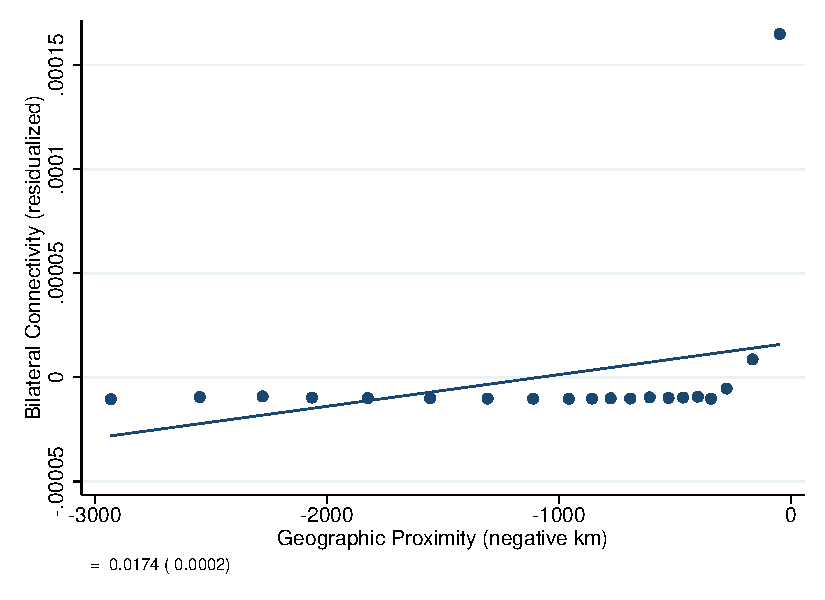
\includegraphics[width=\textwidth]{../Graphs/binscatter_conn_geo_proximity.pdf}
    \caption{Geographic Proximity}
    \label{fig:bin_geo_prox}
\end{subfigure}
\begin{subfigure}{0.49\textwidth}
    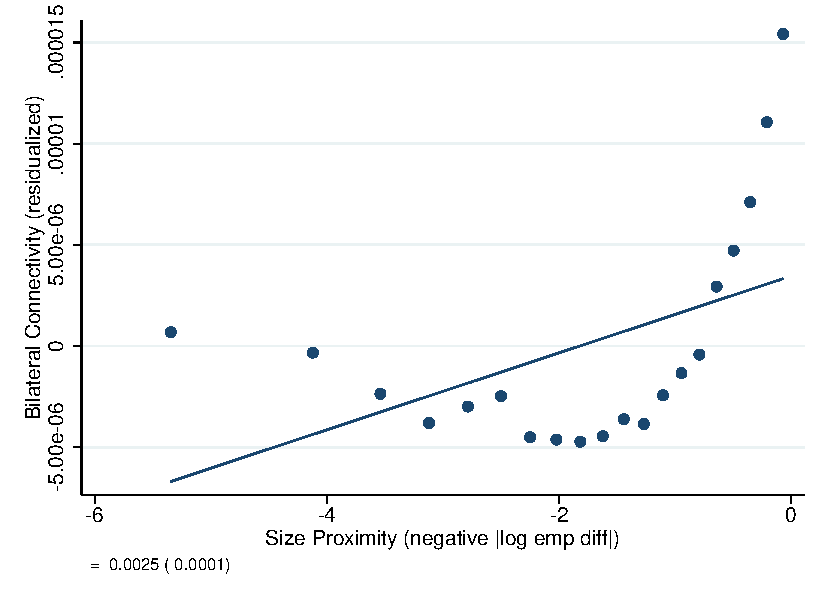
\includegraphics[width=\textwidth]{../Graphs/binscatter_conn_size_proximity.pdf}
    \caption{Size Proximity}
    \label{fig:bin_size_prox}
\end{subfigure}

\begin{subfigure}{0.49\textwidth}
    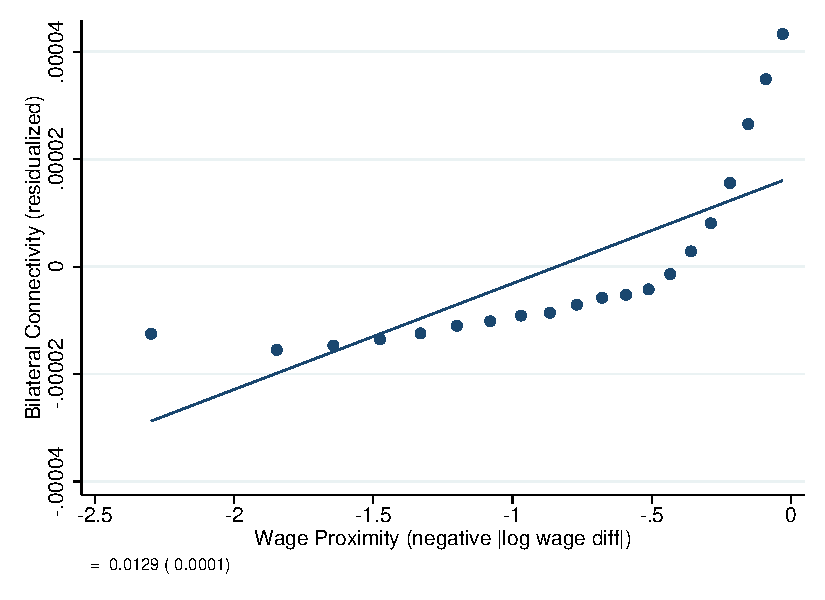
\includegraphics[width=\textwidth]{../Graphs/binscatter_conn_wage_proximity.pdf}
    \caption{Wage Proximity}
    \label{fig:bin_wage_prox}
\end{subfigure}
\begin{subfigure}{0.49\textwidth}
    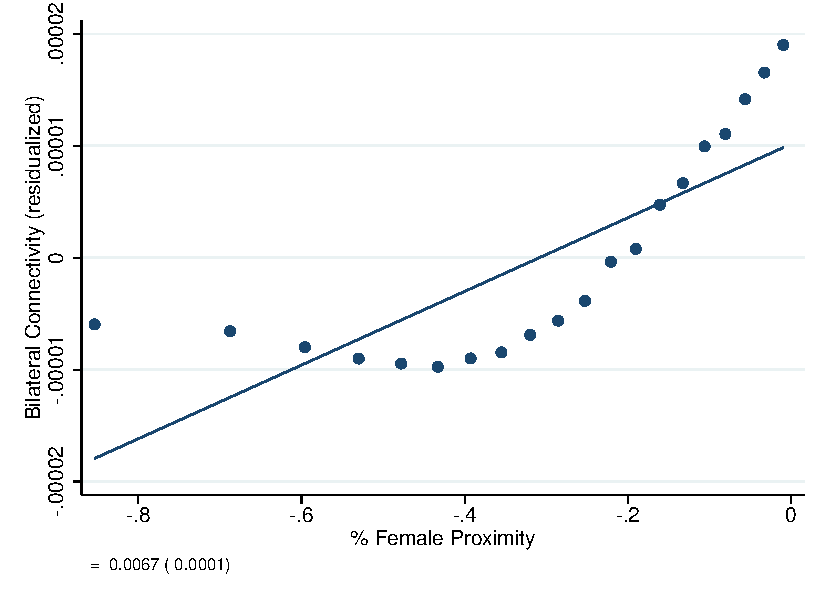
\includegraphics[width=\textwidth]{../Graphs/binscatter_conn_female_proximity.pdf}
    \caption{Share Female Proximity}
    \label{fig:bin_female_prox}
\end{subfigure}

\begin{subfigure}{0.49\textwidth}
    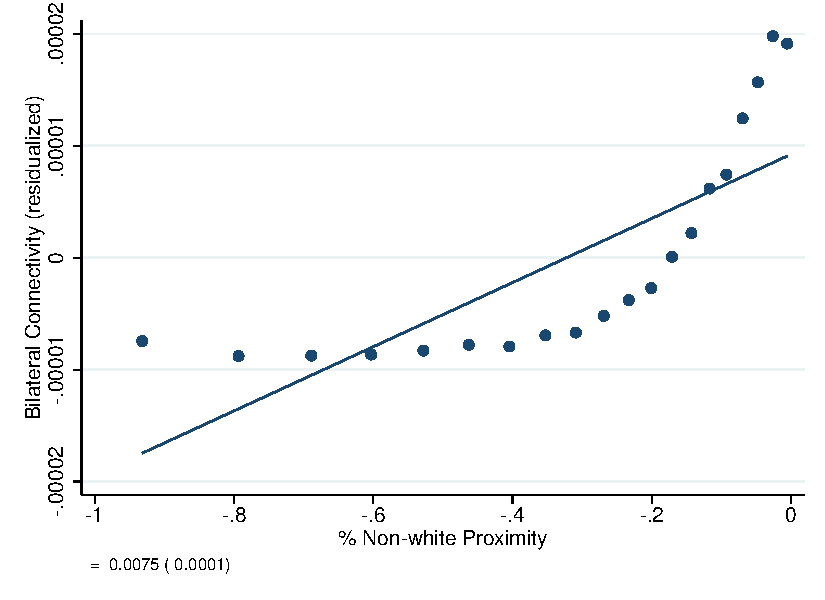
\includegraphics[width=\textwidth]{../Graphs/binscatter_conn_nonwhite_proximity.pdf}
    \caption{Share Non-White Proximity}
    \label{fig:bin_nonwhite_prox}
\end{subfigure}
\begin{subfigure}{0.49\textwidth}
    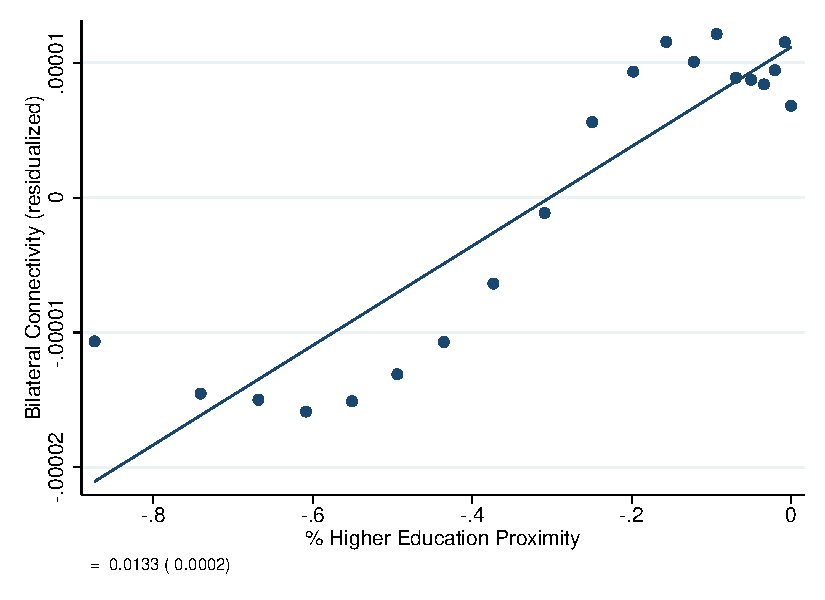
\includegraphics[width=\textwidth]{../Graphs/binscatter_conn_educ_proximity.pdf}
    \caption{Education Proximity}
    \label{fig:bin_educ_prox}
\end{subfigure}

\begin{subfigure}{0.49\textwidth}
    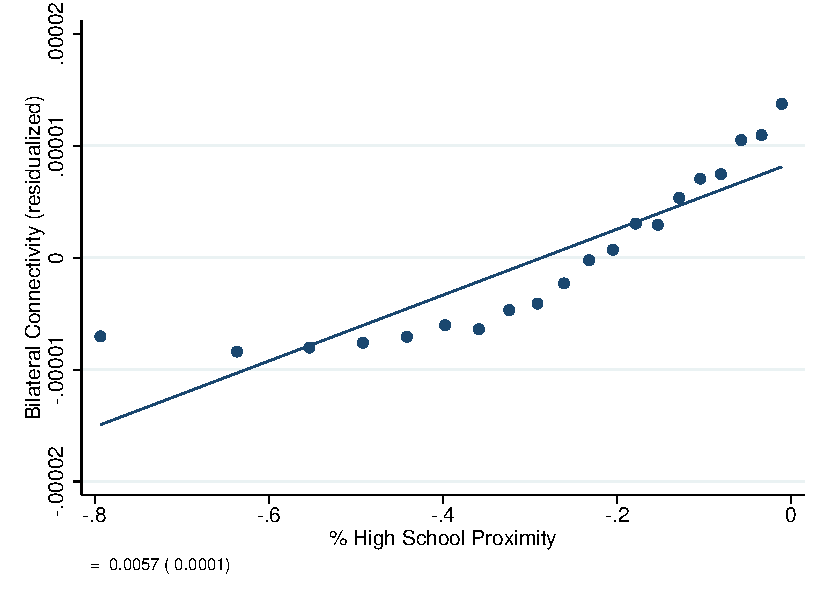
\includegraphics[width=\textwidth]{../Graphs/binscatter_conn_hs_proximity.pdf}
    \caption{High School Proximity}
    \label{fig:bin_hs_prox}
\end{subfigure}
\begin{subfigure}{0.49\textwidth}
    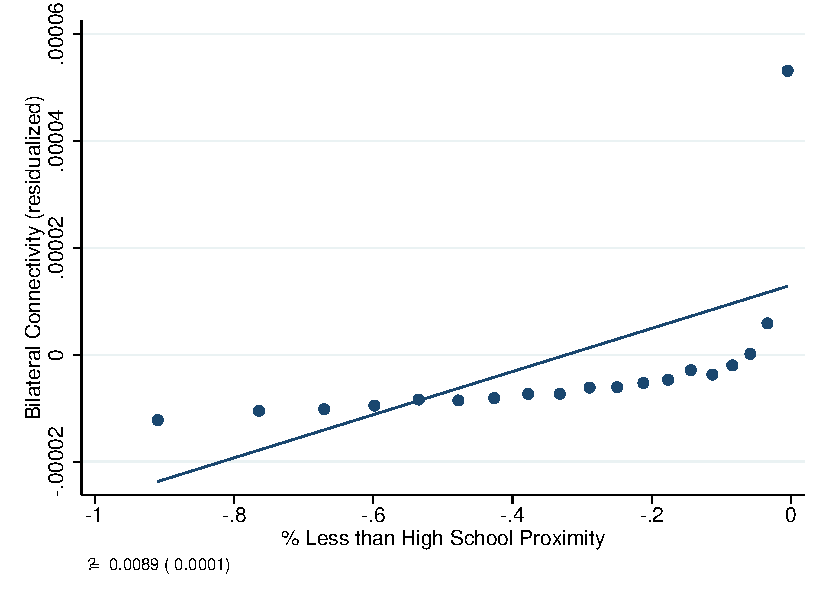
\includegraphics[width=\textwidth]{../Graphs/binscatter_conn_nhs_proximity.pdf}
    \caption{Non-High School Proximity}
    \label{fig:bin_nhs_prox}
\end{subfigure}

\begin{subfigure}{0.49\textwidth}
    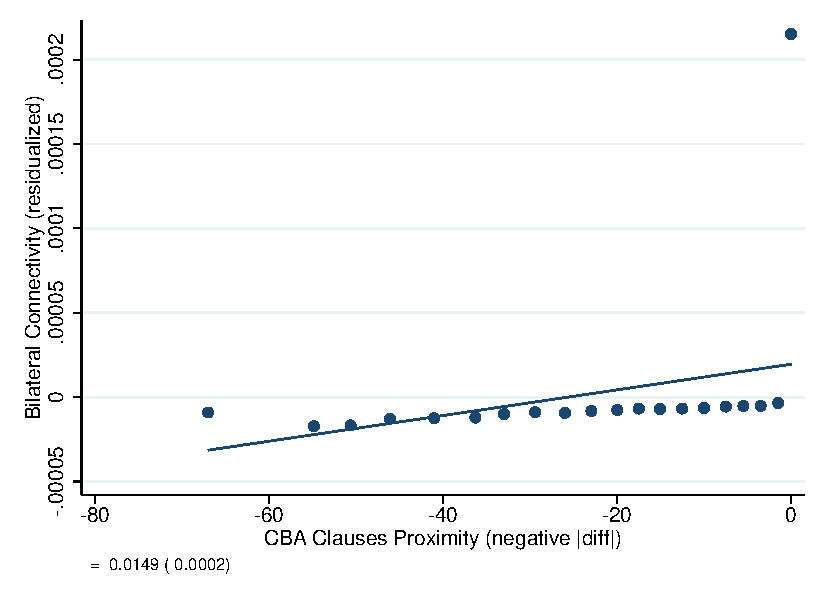
\includegraphics[width=\textwidth]{../Graphs/binscatter_conn_clauses_proximity.pdf}
    \caption{CBA Clauses Proximity}
    \label{fig:bin_clauses_prox}
\end{subfigure}

\caption{Bilateral Connectivity and Establishment Pair Proximity Measures}
\label{fig:binscatters_bilateral}
\begin{tablenotes}
\footnotesize
\item \textit{Notes:} Each panel displays a binned scatterplot of bilateral connectivity against proximity measures between establishment pairs $i$ and $j$. Bilateral connectivity is the average number of worker flows between establishments $i$ and $j$ across consecutive year-pairs (2007-08, 2008-09, 2009-10, 2010-11), normalized by establishment $i$'s employment. Proximity measures are computed as $\text{proximity}_{ij} = 1 - \frac{|x_i - x_j|}{\max_k |x_k - x_l|}$, where higher values indicate greater similarity. Geographic proximity is based on Haversine distance using municipality centroids. Size is average employment over 2009-2011. Wages are median December earnings deflated to 2015 prices. Workforce composition measures (share female, non-white, high school, non-high school, higher education) are averages over 2009-2011. CBA clauses proximity reflects similarity in collective bargaining agreement coverage. Sample includes all establishment pairs where both firms satisfy \texttt{lagos\_sample\_avg==1} and \texttt{in\_balanced\_panel==1}, including pairs with zero bilateral connectivity during 2007-2011.
\end{tablenotes}
\end{threeparttable}
\end{figure}
